\chapter{Analyse et spécification des besoins}

Après avoir posé le contexte et la problématique au chapitre précédent, ce chapitre fait le lien entre ce cadre général et la construction de la plateforme elle-même. Il identifie les acteurs auxquels celle-ci s'adresse et les responsabilités métier qui leur sont associées, avant de spécifier les besoins fonctionnels et non fonctionnels qui en découlent. Une modélisation des cas d'utilisation referme ce chapitre, en formalisant les interactions entre ces acteurs et les principales fonctionnalités de la plateforme, que les chapitres suivants détaillent progressivement.

\section{Analyse des besoins, acteurs et rôles}

Le chapitre précédent a présenté la problématique et les objectifs de ce projet : rapprocher l'évaluation du risque et l'analyse de la rentabilité, au service de la décision d'octroi et du pilotage du portefeuille. Cette section identifie les acteurs auxquels la plateforme s'adresse et les responsabilités métier qui leur sont associées, telles qu'elles sont effectivement prises en charge par la plateforme.

Le \emph{Chargé de clientèle}, responsable de la relation avec les clients qui lui sont affectés, initie les demandes de crédit et en suit le traitement. Il dispose d'un accès aux informations générales, aux décisions et aux revues de risque, mais pas aux données quantitatives du risque, telles que la probabilité de défaut ou les facteurs explicatifs d'une décision, qui relèvent d'une analyse plus spécialisée. L'\emph{Analyste crédit} instruit également les demandes de crédit, mais sur le plan de l'analyse du risque : il dispose, à ce titre, d'un accès aux indicateurs quantitatifs du risque, notamment la probabilité de défaut, la perte en cas de défaut, les pertes attendues et les facteurs explicatifs d'une décision, en plus des éléments déjà accessibles au Chargé de clientèle.

Le \emph{Risk Manager} occupe une position centrale dans le dispositif : il valide les décisions de crédit qui dépassent le seuil délégué aux deux acteurs précédents, intervient dans les décisions prises en comité de crédit, et pilote l'analyse du portefeuille (risque, pertes, capital, rentabilité) dans la durée. Son accès aux données de la plateforme est, en conséquence, le plus complet.

La \emph{Direction} dispose d'un accès en lecture à des synthèses agrégées de portefeuille et à des indicateurs stratégiques, sans intervenir dans le traitement d'un dossier individuel ni dans les décisions d'octroi. La \emph{Conformité et l'Audit} consultent a posteriori les décisions prises et leur traçabilité, afin d'en contrôler la cohérence, sans participer eux-mêmes à ces décisions. L'\emph{Administrateur}, enfin, gère les aspects techniques de la plateforme (utilisateurs, rôles et configuration). Ses responsabilités relèvent de l'administration du système. Il ne dispose pas du pouvoir de validation individuelle des crédits, mais peut intervenir dans le processus collégial de décision en comité, conformément aux autorisations prévues dans la plateforme.

Le tableau~\ref{tab:acteurs-roles} résume ces responsabilités et leur correspondance avec les rôles effectivement définis dans la plateforme.

\begin{table}[htbp]
    \centering
    \footnotesize
    \caption{Acteurs de la plateforme et responsabilités principales.}
    \label{tab:acteurs-roles}
    \begin{tabular}{p{3.2cm}p{7cm}p{3.5cm}}
        \toprule
        \textbf{Acteur} & \textbf{Responsabilités principales} & \textbf{Rôle correspondant} \\
        \midrule
        Chargé de clientèle & Initie et suit les demandes de crédit de ses clients. & \texttt{RELATIONSHIP\_MGR} \\
        \addlinespace
        Analyste crédit & Instruit les demandes de crédit et en analyse le risque. & \texttt{CREDIT\_ANALYST} \\
        \addlinespace
        Risk Manager & Valide les décisions, décide en comité de crédit, pilote le portefeuille. & \texttt{RISK\_MANAGER} \\
        \addlinespace
        Direction & Consulte des synthèses stratégiques agrégées du portefeuille. & \texttt{EXECUTIVE} \\
        \addlinespace
        Conformité / Audit & Contrôle a posteriori la traçabilité des décisions. & \texttt{COMPLIANCE\_AUDIT} \\
        \addlinespace
        Administrateur & Gère les aspects techniques de la plateforme. & \texttt{ADMIN} \\
        \bottomrule
    \end{tabular}
\end{table}

\section{Spécification des besoins fonctionnels}

\subsection{Gestion des demandes de crédit (Origination)}

Les acteurs intervenant dans le processus d'octroi, le Chargé de clientèle et l'Analyste crédit, doivent pouvoir saisir une nouvelle demande de crédit, l'instruire avec les informations nécessaires à son évaluation, puis accéder à une décision d'octroi justifiée, assortie des éléments de risque et de rentabilité qui la motivent.

\subsection{Évaluation du risque et des pertes}

La plateforme doit produire les indicateurs quantitatifs nécessaires à l'analyse du risque, à la fois pour un dossier individuel lors de son instruction, et pour un portefeuille de crédits déjà accordés lors de son suivi, sans que ces deux évaluations reposent nécessairement sur les mêmes mécanismes de calcul. Pour un dossier individuel, ce besoin consiste à évaluer le risque de l'emprunteur et à estimer les pertes attendues et le capital pris en compte dans l'analyse, selon les mécanismes retenus pour l'Origination. Pour un portefeuille, il consiste à analyser les pertes attendues et le capital mobilisé à l'échelle du portefeuille, en tenant compte de son exposition globale.

\subsection{Analyse et pilotage du portefeuille (Portfolio Analytics)}

Le Risk Manager doit pouvoir suivre l'évolution du portefeuille dans le temps et en analyser les principales caractéristiques, à partir des indicateurs produits par l'évaluation du risque. La Direction doit, quant à elle, disposer d'une vision synthétique et agrégée de cette évolution.

\subsection{Analyse du capital, de la rentabilité et aide à la décision}

La plateforme doit mettre en relation le risque, les pertes attendues, le capital et la rentabilité, afin d'éclairer, d'une part, la décision d'octroi d'un dossier individuel, notamment lors des validations et des interventions en comité de crédit prévues par les seuils de délégation présentés en section~2.1, et, d'autre part, le pilotage du portefeuille dans son ensemble.

\subsection{Assistant intelligent}

La plateforme doit permettre aux utilisateurs d'interroger, en langage naturel, les informations et résultats qu'elle produit, dans les limites des données et des fonctionnalités auxquelles leur rôle leur donne accès. Cet assistant reste une fonctionnalité consultative : il n'intervient dans aucune décision et ne garantit pas de répondre à toute question qui lui est posée.

\section{Spécification des besoins non fonctionnels}

\subsection{Sécurité et contrôle d'accès}

Chaque utilisateur ne doit accéder qu'aux fonctionnalités correspondant à son rôle, et qu'aux données couvertes par les autorisations associées à ce rôle, selon la répartition des responsabilités présentée en section~2.1.

\subsection{Traçabilité et auditabilité}

La plateforme doit assurer la traçabilité des traitements et des décisions significatifs, notamment les opérations d'ingestion, de transformation, d'entraînement et de décision de crédit. Les événements enregistrés doivent pouvoir être vérifiés a posteriori, et leur intégrité doit être protégée contre toute modification silencieuse.

\subsection{Fiabilité et cohérence des calculs}

Les résultats produits doivent respecter la cohérence des relations entre les indicateurs de risque, les pertes attendues, le capital et la rentabilité. Les calculs doivent également être reproductibles à partir des mêmes données et des mêmes paramètres.

\subsection{Gestion des volumes de données}

La plateforme doit pouvoir traiter les données des segments Particuliers et Entreprises dans des délais compatibles avec les traitements périodiques prévus pour l'évaluation du risque et le suivi du portefeuille.

\subsection{Modularité et maintenabilité}

Les composants d'évaluation du risque, de quantification financière et d'aide à la décision doivent pouvoir évoluer indépendamment les uns des autres.

\section{Modélisation des cas d'utilisation}

La figure~\ref{fig:cas-utilisation} présente les interactions entre les six acteurs identifiés en section~2.1 et les principales fonctionnalités de la plateforme, regroupées en cinq ensembles fonctionnels correspondant aux principaux parcours de la plateforme : l'évaluation d'une demande de crédit (Origination), l'arbitrage et le comité de crédit, l'analyse du portefeuille (Portfolio Analytics), la gouvernance et l'audit, et l'assistant conversationnel, transversal aux six acteurs. Les associations entre acteurs et cas d'utilisation reflètent directement les autorisations réellement définies dans la plateforme.

\begin{figure}[htbp]
    \centering
    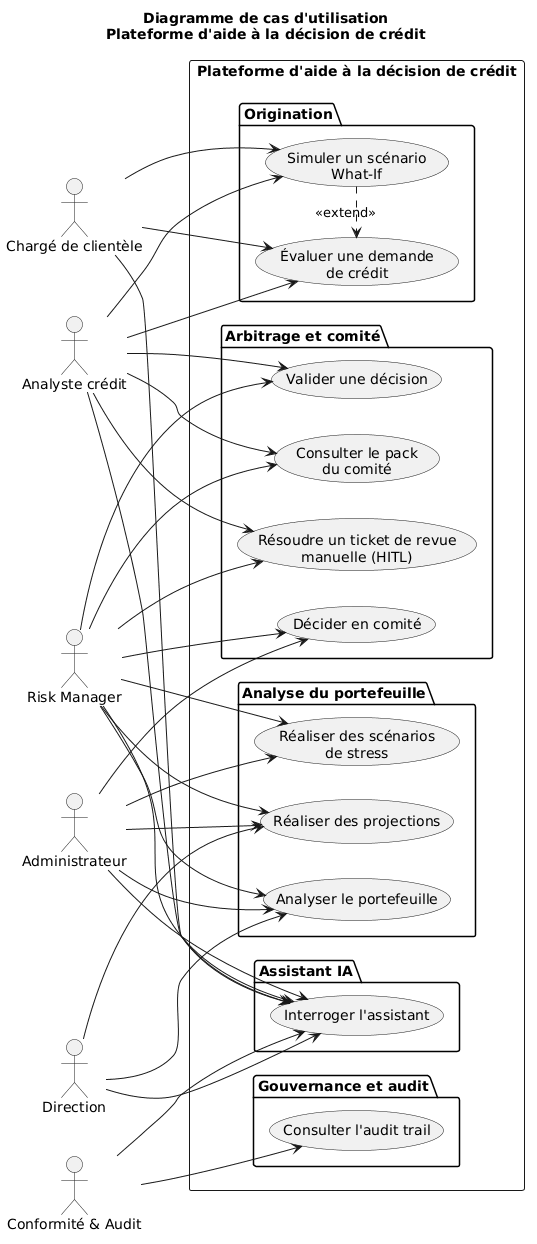
\includegraphics[width=\textwidth,height=0.85\textheight,keepaspectratio]{figures/diagramme_cas_utilisation_v2.png}
    \caption{Diagramme de cas d'utilisation de la plateforme (élaboration personnelle, à partir des rôles et autorisations réellement implémentés).}
    \label{fig:cas-utilisation}
\end{figure}

Parmi ces cas d'utilisation, quatre concentrent l'essentiel de la valeur métier de la plateforme et sont décrits plus en détail dans le tableau~\ref{tab:cas-utilisation-prioritaires}.

\begin{table}[htbp]
    \centering
    \footnotesize
    \caption{Description des cas d'utilisation prioritaires.}
    \label{tab:cas-utilisation-prioritaires}
    \begin{tabular}{p{3cm}p{3cm}p{8cm}}
        \toprule
        \textbf{Cas d'utilisation} & \textbf{Acteur(s)} & \textbf{Description} \\
        \midrule
        Évaluer une demande de crédit &
        Chargé de clientèle, Analyste crédit &
        Saisir une nouvelle demande de crédit et en obtenir l'évaluation du risque, jusqu'à une décision d'octroi justifiée. Ce cas d'utilisation peut être étendu par la simulation d'un scénario \emph{What-If}, qui permet de recalculer cette évaluation pour des paramètres de la demande modifiés par l'utilisateur, sans enregistrer le résultat dans le système. \\
        \addlinespace
        Valider une décision / Décider en comité &
        Risk Manager (validation seule) ; Risk Manager et Administrateur (décision en comité) &
Statuer sur les demandes dont la décision dépasse le niveau de délégation accordé au Chargé de clientèle et à l'Analyste crédit. Une décision individuelle est validée par le Risk Manager seul ; une décision collégiale, prise en comité de crédit, peut associer l'Administrateur à la décision du Risk Manager. \\
        \addlinespace
        Résoudre un ticket de revue manuelle &
        Analyste crédit, Risk Manager &
        Traiter un dossier signalé pour un examen humain (par exemple une incohérence ou une limite atteinte par l'évaluation automatisée), jusqu'à sa résolution. \\
        \addlinespace
        Analyser le portefeuille &
        Risk Manager, Direction &
        Consulter l'évolution du risque, des pertes attendues, du capital mobilisé et de la rentabilité d'un portefeuille de crédits déjà accordés, notamment à travers des projections et des scénarios de stress. \\
        \bottomrule
    \end{tabular}
\end{table}

\section*{Conclusion du chapitre}

Ce chapitre a traduit le cadrage posé au chapitre précédent en besoins concrets. Six acteurs ont été identifiés, chacun avec des responsabilités et des droits d'accès qui lui sont propres, de l'instruction d'une demande de crédit au contrôle a posteriori des décisions prises. Les besoins fonctionnels couvrent les deux volets de la plateforme, Origination et Portfolio Analytics, ainsi que l'assistant intelligent qui les accompagne ; les besoins non fonctionnels portent sur la sécurité, la traçabilité, la fiabilité des calculs, les volumes de données et la maintenabilité des composants. La modélisation des cas d'utilisation a permis de représenter ces besoins sous la forme des interactions réellement autorisées entre les acteurs et la plateforme. Le chapitre suivant aborde la préparation des données et la construction des modèles prédictifs qui contribuent à l'évaluation du risque.
